%%%%%%%%%%%%%%%%%%%%%%%%
%
% $Autor: Gautam Ramesh$
% $Datum: 2025-10-14 12:26:42Z $
% $Pfad: /Users/gautamramesh/githubNew/ML26-03-Car-Licence-Plate-Identification-with-a-Jetson-Nano/Assembly - edit/Chapters/en/SetUp.tex $
% $Version: 4251 $
%
% !TeX encoding = utf8
% !TeX root = Rename
%
%%%%%%%%%%%%%%%%%%%%%%%%

\chapter{Setup}

This chapter walks you through preparing the microSD card, assembling the hardware, completing the first boot configuration, and validating the camera and display. Follow the steps in order and use the checklists to prevent common mistakes.

\section{Before You Begin}

\subsection*{Workspace and Safety}
\begin{itemize}
	\item Work on a clean, non-conductive surface with good lighting.
	\item Avoid electrostatic discharge (ESD): touch a grounded metal object before handling the board.
	\item Keep cables short and routed to avoid strain on connectors.
\end{itemize}

\subsection*{You Will Need}
\begin{itemize}
	\item NVIDIA Jetson Nano (4~GB, B01).
	\item \SI{32}{\giga\byte} microSD card (UHS-I, Class~10) prepped with JetPack~5.1.2.
	\item Official \SI{5}{\volt}, \SI{4}{\ampere} DC power adapter (barrel jack).
	\item USB camera (UVC compliant; e.g., Microsoft LifeCam Show).
	\item HDMI monitor + HDMI cable.
	\item USB keyboard and mouse (wired or 2.4\,GHz dongle).
\end{itemize}

\begin{quote}\small
	\textbf{Tip.} Faster microSD media (high sustained write, UHS-I) noticeably improves system responsiveness and logging performance.
\end{quote}

\section{Prepare the microSD Card}

\subsection*{Download and Flash}
\begin{enumerate}
	\item Download the Jetson Nano image for JetPack~5.1.2 from NVIDIA.
	\item Use a flashing tool (e.g., Raspberry Pi Imager or balenaEtcher) to write the image to the \SI{32}{\giga\byte} microSD card.
	\item After flashing completes, safely eject the card.
\end{enumerate}

\begin{figure}[H]
	\centering
	% Place your own screenshots in General/Images/...
	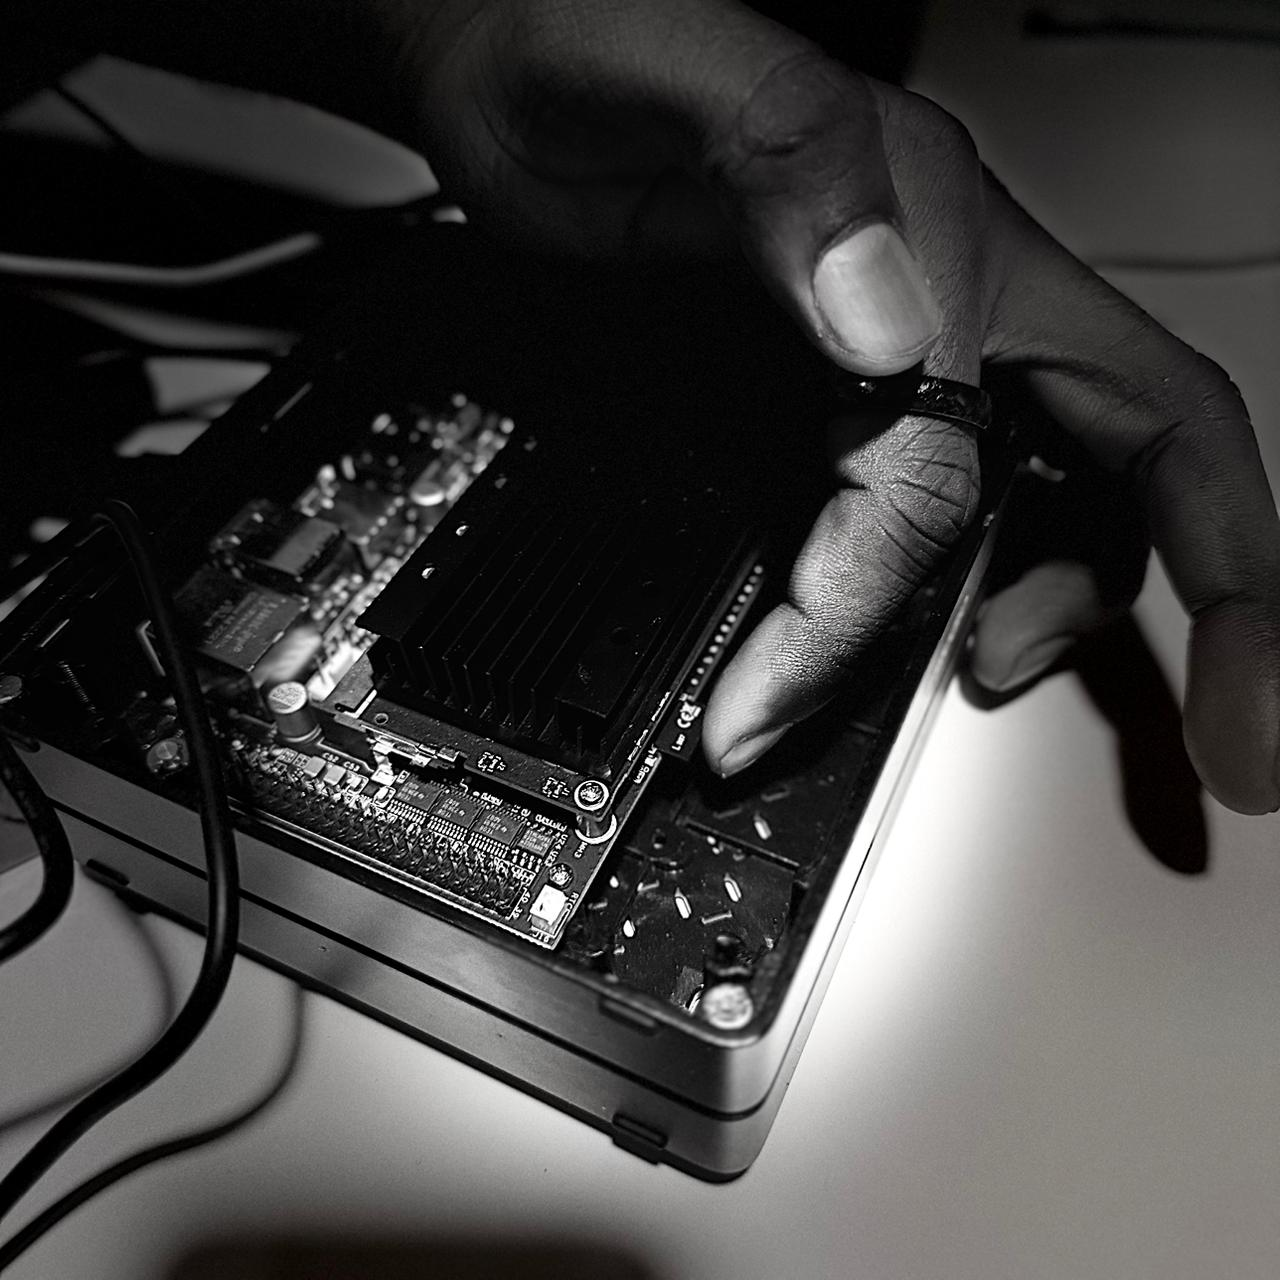
\includegraphics[width=.85\linewidth]{images/SdCard.jpeg}
	\caption{Flashing JetPack image to microSD using a cross-platform imager.}
	\label{fig:sd-flash}
\end{figure}

\begin{quote}\small
	\textbf{Note.} If you maintain a “known-good” cloned card, you can swap cards to recover quickly without re-imaging.
\end{quote}

\section{Hardware Assembly}

\subsection*{Install and Connect}
\begin{enumerate}
	\item Insert the flashed microSD card into the Jetson Nano microSD slot.
	\item Connect the HDMI cable from the Jetson to the monitor.
	\item Plug in the USB camera to a USB~3.0 port (prefer the blue receptacle).
	\item Connect keyboard and mouse (separate USB ports, or a receiver dongle).
	\item \emph{Do not} power the board yet.
\end{enumerate}

\begin{figure}[H]
	\centering
%	
\includegraphics[width=.9\linewidth]{images/jetsonTopLayout.jpg}
	\caption{Jetson Nano top layout with key ports. Use short, good-quality cables.}
	\label{fig:jetson-top}
\end{figure}

\begin{figure}[H]
	\centering
	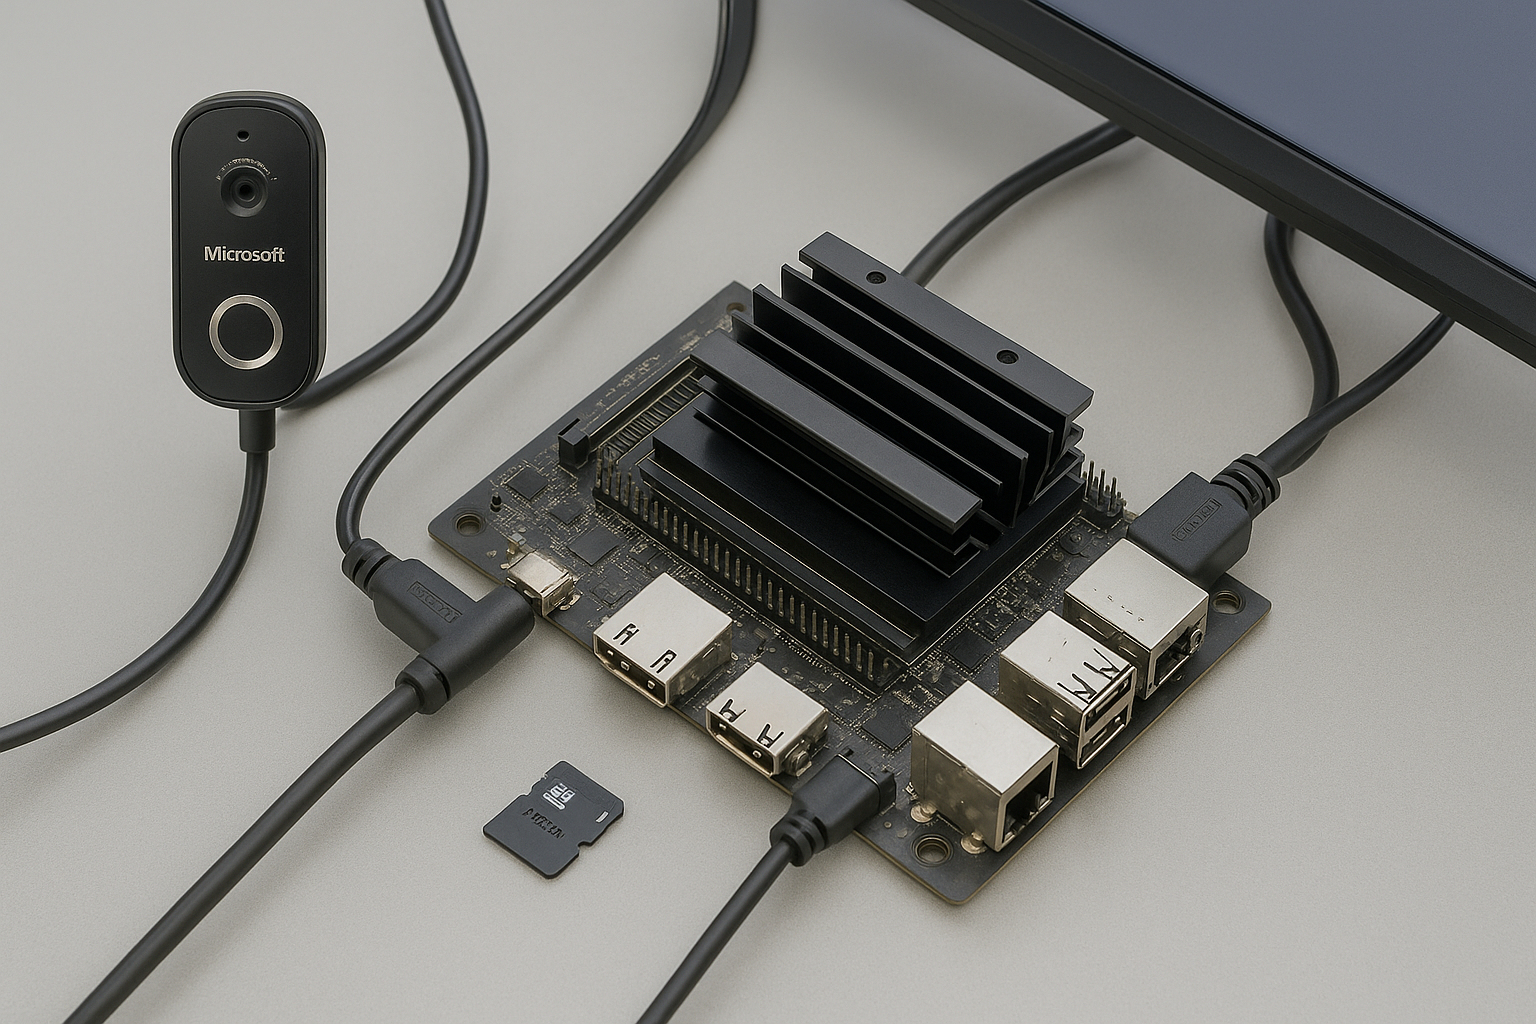
\includegraphics[width=.9\linewidth]{images/wiringOverview.png}
	\caption{Wiring overview: USB camera, HDMI to monitor, keyboard/mouse, and DC barrel power.}
	\label{fig:wiring-overview}
\end{figure}

\begin{quote}\small
	\textbf{Warning.} Only use a regulated \SI{5}{\volt}, \SI{4}{\ampere} adapter. Underrated supplies can cause throttling or brownouts.
\end{quote}

\section{First Boot Configuration}

\subsection*{Power On and Wizard}
\begin{enumerate}
	\item Connect the \SI{5}{\volt} adapter to the DC barrel jack to power on.
	\item Complete the first-boot wizard: locale, keyboard, user account, and display settings.
	\item Verify the monitor is set to the correct HDMI input.
\end{enumerate}

\subsection*{Recommended System Settings}
From a terminal:
\begin{verbatim}
	# Performance mode and clocks (Jetson Nano)
	sudo nvpmodel -q         # Check current mode
	sudo nvpmodel -m 0       # Max performance profile
	sudo jetson_clocks       # Lock clocks for consistent benchmarking
\end{verbatim}

(Optional) Create swap to improve stability during large installs:
\begin{verbatim}
	# Create a 2 GB swapfile
	sudo fallocate -l 2G /swapfile
	sudo chmod 600 /swapfile
	sudo mkswap /swapfile
	sudo swapon /swapfile
	# Make persistent:
	echo '/swapfile none swap sw 0 0' | sudo tee -a /etc/fstab
\end{verbatim}

\section{Camera and Display Validation}

\subsection*{Detect the Camera}
\begin{verbatim}
	lsusb
	v4l2-ctl --list-devices
	v4l2-ctl --list-formats-ext -d /dev/video0
\end{verbatim}

\subsection*{Live Preview (USB UVC Camera)}
\begin{verbatim}
	# GStreamer preview (generic UVC):
	gst-launch-1.0 v4l2src device=/dev/video0 ! videoconvert ! autovideosink
\end{verbatim}

\subsection*{HDMI Output Sanity Check}
\begin{verbatim}
	xrandr            # Confirm HDMI mode
\end{verbatim}

If the monitor remains blank, reseat the HDMI cable and ensure the correct input source is selected.

\section{Software Prerequisites (Minimal)}

\subsection*{Base Tools}
\begin{verbatim}
	sudo apt update
	sudo apt install -y python3-pip python3-venv git \
	gstreamer1.0-tools v4l-utils
\end{verbatim}

\subsection*{Python Environment (Optional but Recommended)}
\begin{verbatim}
	python3 -m venv ~/lpd-venv
	source ~/lpd-venv/bin/activate
	pip install --upgrade pip
	# install your project requirements afterwards, e.g.:
	# pip install opencv-python numpy onnxruntime easyocr
\end{verbatim}

\section{Quick Setup Checklist}

\begin{table}[H]
	\centering
	\caption{Setup Checklist}
	\begin{tabular}{|L{7.2cm}|L{6.0cm}|}
		\hline
		\textbf{Task} & \textbf{Status / Notes} \\ \hline
		microSD flashed with JetPack~5.1.2 & \rule{4cm}{0.4pt} \\ \hline
		HDMI connected, monitor input selected & \rule{4cm}{0.4pt} \\ \hline
		USB camera detected as \texttt{/dev/video0} & \rule{4cm}{0.4pt} \\ \hline
		Keyboard/mouse functional on login & \rule{4cm}{0.4pt} \\ \hline
		Performance mode enabled (\texttt{nvpmodel -m 0}) & \rule{4cm}{0.4pt} \\ \hline
		Live camera preview verified (GStreamer) & \rule{4cm}{0.4pt} \\ \hline
	\end{tabular}
\end{table}

\section{Troubleshooting Hints (Setup Phase)}

\begin{itemize}
   \item \textbf{No display:} Check HDMI input source; try a different cable; test at 1920×1080 resolution first.
	\item \textbf{Camera not found:} Try a different USB port; confirm with \texttt{v4l2-ctl}; ensure the camera is UVC compliant.
	\item \textbf{Random freezes:} Use the official \SI{5}{\volt}/\SI{4}{\ampere} PSU; enable swap; keep cables short.
	\item \textbf{Laggy UI:} Prefer a faster microSD card; avoid heavy desktop compositing during inference.
	\item \textbf{No boot or LED activity:} Verify that the power supply provides a stable \SI{5}{\volt} output; reseat the microSD card and ensure correct image flashing using \texttt{balenaEtcher}.
	\item \textbf{No USB response:} Avoid using low-quality USB hubs; check for sufficient power on all ports; test individual peripherals directly on the Nano.
	\item \textbf{HDMI signal drop or flicker:} Use a certified high-speed HDMI cable shorter than 1.5\,m; ensure the monitor is set to digital input mode.
	\item \textbf{Camera lag or frame skipping:} Reduce resolution to 720p or lower; close background processes; verify USB 3.0 port usage.
	\item \textbf{System not connecting to network:} Confirm Ethernet link LEDs; check IP assignment using \texttt{ifconfig}; reset network settings if required.
	\item \textbf{Thermal throttling or sudden shutdowns:} Clean the heatsink and ensure the fan spins freely; use passive cooling pads for long runs.
	\item \textbf{microSD not detected:} Ensure the card is fully seated and formatted as FAT32 before flashing; avoid counterfeit cards from unknown vendors.  
	\item \textbf{Peripheral power loss:} If multiple USB devices disconnect randomly, use a powered USB hub to offload current from the Nano’s onboard regulator.  
	\item \textbf{Unstable camera preview:} Check exposure settings under \texttt{v4l2-ctl}; excessive ambient light or glare may cause false negatives during detection.  
	\item \textbf{Frequent file corruption:} Always perform a safe shutdown (\texttt{sudo poweroff}) to avoid SD-card write failure; consider switching to an SSD for better endurance.  
	\item \textbf{Inconsistent detection results:} Clean the camera lens; verify that lighting and plate angle match the trained dataset conditions for YOLOv8 and EasyOCR accuracy.  
\end{itemize}
